\chapter{Super-Kamiokande Detector Calibration}
\label{chp:superkcalib}

In order to achieve optimal event reconstruction for physics analyses, calibration of the Super-Kamiokande detector is crucial. For example, when conducting Monte Carlo simulations of certain processes in the detector, facets of the experiment such as properties of the water, photomultiplier tube response and the inner detector and outer detector electronics are all calibrated so that input parameters for the Monte Carlo simulations can be obtained. This chapter will concern itself with the inner and outer detector calibration, including photomultiplier tube and electronics calibration, PMT gain calibration, quantum efficiency determination and hit timing and charge information calibration. 

\section{Inner detector calibration}

\subsection{PMT High-voltage setting calibration}

The high-voltage (HV) setting for all photomultiplier tubes need to adjusted individually so all the PMTs produce the same amount of charge for a certain light intensity recieved by them. Placing a light source which distributes light isotropically in the centre of the inner detetector to achieve this calibration means that there is no position in the detector from which the inner detector PMTs are equidistant, so each PMT will not recieve the same amount of light from the light source. To avoid this problem, a set of 420 pre-calibrated PMTs inside the detector were used, seperated into groups relating to their geometrical distance from the HV calibration light source (see Figure \ref{fig:hvcalib} for their location with respect to the other photomultiplier tubes.)

\begin{figure}
    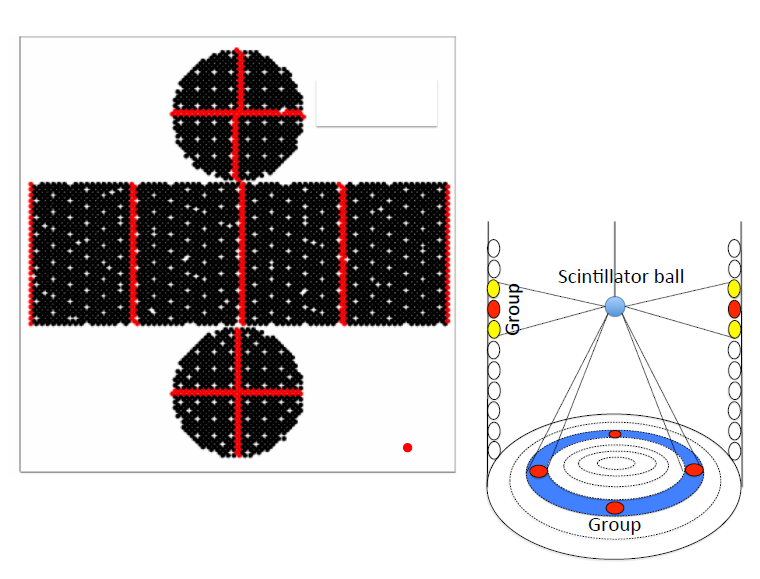
\includegraphics[width=\textwidth]{Figures/hvcalib.png}
\caption{Location of 420 reference PMTs used for HV setting calibration. The red lines in show the placement of these PMTs with repsect to the others (left). The grouping of these PMTs due to their geometry in relation to the light source is also shown (right) }
    \label{fig:hvcalib}
\end{figure}




\subsection{Relative gain calibration}

Understanding the timing information from the hit photomultiplier tubes depends on how well the charge from the hit PMT is calculated. To conceive charge calibration, a quantity called photomultiplier tube ''gain" must be calculated. ''Gain" is the conversion factor from the number of photoelectrons produced by the hit PMT and charge, and calibration of this quantity is what interpretation of very high energy events (TeV scale) rely on. Quantum efficiency is another quantity used for the calibration of low energy physics events (such as detection of solar neutrinos), due to them consisting of single photoelectron (single-pe) hits: it is the ratio of the number of the number of photoelectrons emitted by the cathode to the number of photons that are incident on the photomultiplier tube window. Super-Kamiokande calibration converts this measure of quantum efficiency into ''QE" by multiplying the quantum efficiency by the collection efficiency of the photoelectrons onto the first dynode inside the PMT \cite{abe_calibration_2014}. Knowing the gain and QE of each PMT in the detector is important in order to accurately measure the output charge from each individual PMT, which is done by first calculating the relative gain difference among all PMTs and then work out the average gain difference over all PMTs in the detector. After this, the variation away from this average gain value can be calculated for each seperate inner detector photomultiplier tube, and the gain value for each can be extracted. 

The relative gain difference is calculated by two measurements using a light source to produce constant-intensity flashes. The first measurement involves using the light source to produce high-intensity flashes so that all photomultiplier tubes in the detctor gets a certain number of photons, and the second measurement has the light source produce low-intensity flashes so that only a few PMTs are hit. The first measurement provides an average charge value ($Q_{o b s}(i)$) for each inner detector PMT, while the second measurement gives single photoelectron hits, providing a number of times ($N_{o b s}(i)$) that a single PMT gives a charge which is greater than the PMT threshold value. Equation \ref{eq:gaineq} shows how these two values are calculated from the the high and low intensity flash values ($I$), the acceptance of the PMT(i) ($a(i)$), the QE value of the PMT ($\varepsilon_{q e}$) and the PMT gain $G$. 

\begin{align}
Q_{o b s}(i) \quad \propto \quad I_{high} \times a(i) \times \varepsilon_{q e}(i) \times G(i) \\
N_{o b s}(i) \quad \propto \quad I_{low} \times a(i) \times \varepsilon_{q e}(i)
\end{align}
\label{eq:gaineq}

Therefore, by simply dividing these two values of $Q_{o b s}(i)$ and ($N_{o b s}(i)$) the average gain over all PMTs can be calculated.  Figure \ref{fig:relativegain} shows the spread of the relative gain over all the PMTs. 

\begin{figure}
    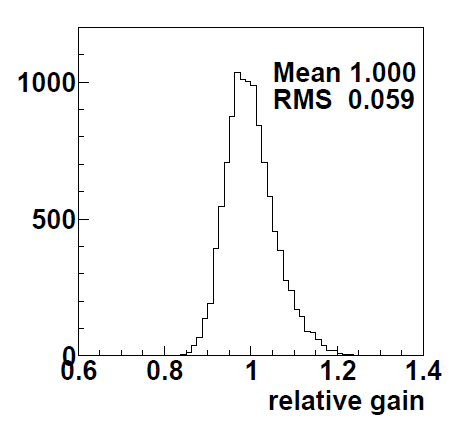
\includegraphics[width=\textwidth]{Figures/relativegain.png}
\caption{Relative gain of PMTs in Super-Kamiokande}
    \label{fig:relativegain}
\end{figure}

\subsection{Absolute gain calibration}

In order to calculate absolute gain, the single photoelectron distrubution needs to be measured, this is because absolute gain relates to the observed charge in the photomultplier tube with the number of photoelectrons produced. A nickel-californium source (shown in Figure \ref{fig:nickel_source}) is used for this measurement due to it releasing gamma rays isotropically. Thermal neutron capture on nickel is used as the gamma ray source, with the neutrons provided by the spontaneous fission of ${ }^{252} \mathrm{Cf}$. This nickel source is placed in the centre of the inner detector and the gamma rays produced are detetced by all the inner detector PMTs. On average the observed number of photoelectrons is 0.004 per event per PMT, meaning that single p.e. hits are observed for more than 99\% of the hits. The observed charge distribution of all the hits from this nickel source is used to give the average charge, which is used as a conversion factor from a charge measurement in picoColoumbs and single photo-electrons. The factor is 2.658pC per photoelectron (calculated at the beginning of SK-IV) which is then used to extract the single-p.e. distribution, shown in Figure \ref{fig:singlepe}.

\begin{figure}
    \centering
    \begin{subfigure}[b]{.5\textwidth}
      \centering
      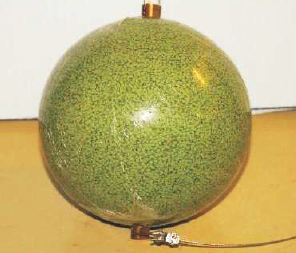
\includegraphics[width=.7\linewidth]{Figures/nickel_source.png}
      \caption{Photograph of nickel source}
      \label{fig:nickel_source}
    \end{subfigure}
    \hskip -1ex
    \begin{subfigure}[b]{.5\textwidth}
      \centering
      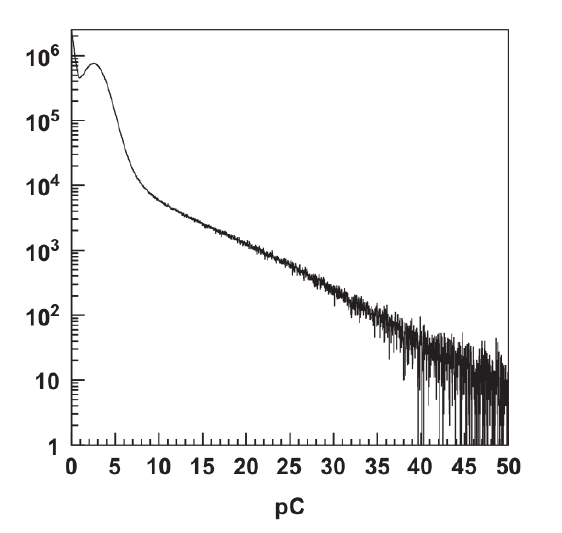
\includegraphics[width=.7\linewidth]{Figures/singlepe.png}
      \caption{Single p.e distribution of charge in pC}
      \label{fig:singlepe}
    \end{subfigure}
    \end{figure}
    

\begin{figure}
    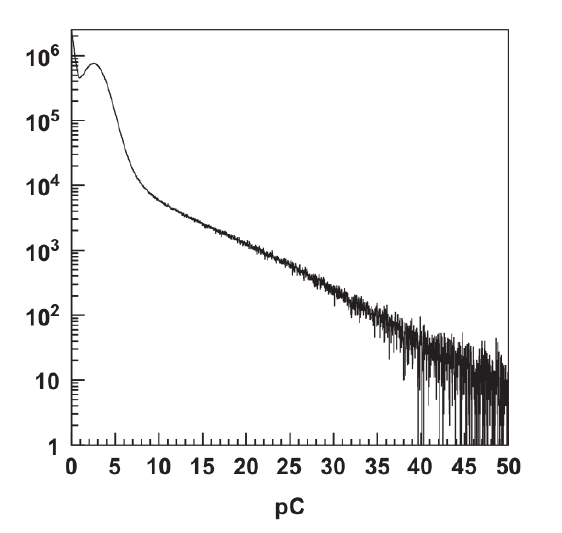
\includegraphics[width=\textwidth]{Figures/singlepe.png}
\caption{Single p.e distribution of charge in pC }
    \label{fig:singlepe}
\end{figure}
    

\subsection{Relative quantum efficiency measurement}

To measure the relative quantum efficiency, the gamma rays from neutron capture on the nickel source are simulated. Inside this simulation, a common value of QE is used for all the ID PMTs to predict the number of hits for each PMT. Comparing this number of hits to the actual data obtained for each individual PMT by calculating the ratio between them provides us with a value for relative QE for each inner detetor PMT which is then used inside the simulation. 

\subsection{Timing information calibration}
Calibrating the hit timing information of the photomultiplier tubes is essential due to its importance in accurately being able to reconstruct events. Event reconstruction makes use of determining exactly where interaction vertices are and the direction in which particles travel, and to do this the time response needs to be very carefully calibrated. The response time of the PMT also relates to the amount of charge observed: in order for a hit to be registered, the PMT signal must pass the discriminator value of the hit threshold, and the time in which this happens is dependent on height of the pulse, which is correlated with observed charge. All thsese factors need to be considered when calibrating hit timing information.
\newline
To aid the timing calibration, a diffuser ball is placed near the centre of the inner detector, into which a nitrogen laser injects pulsed laser light. By varying the intensity of this light, the laser light can be outputted in flashes, and the timing of the laser pulses is monitored using a 2-inch monitor PMT. The schematic of this timing calibration system is shown in Figure \ref{fig:timecalibsystem}.

\begin{figure}
    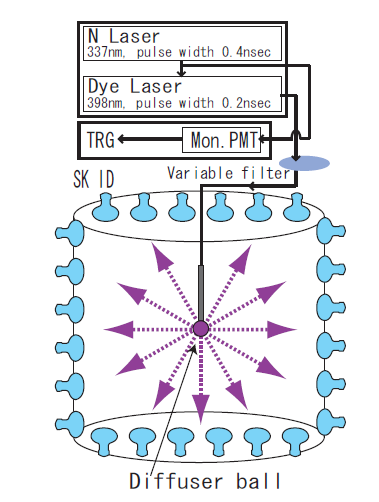
\includegraphics[width=\textwidth]{Figures/timecalibsystem.png}
\caption{Schematic of timing calibration system, with SK ID PMTs in blue and the diffuser ball in purple. The dye laser shifts the wavelength of the laser light to 398 nm to maximise the quantum efficiency of the PMTs and light absorption.}
    \label{fig:timecalibsystem}
\end{figure}


The value of these laser pulse timings, and the time-of-flight value from the diffuser ball are subtracted from the PMT hit time. Using the observed charge values and these adjusted hit times, "TQ" (time and charge) distributions can be plotted for each inner detetector PMT. An example TQ distribution is shown for an inner detector PMT (cable number 00010) in Figure \ref{fig:TQdist}, where the vertical axis shows is the TOF corrected and laser pulse time corrected PMT hit time, the horizontal axis shows the observed charge of each hit. Figure taken from \cite{abe_calibration_2014}. 

\begin{figure}
    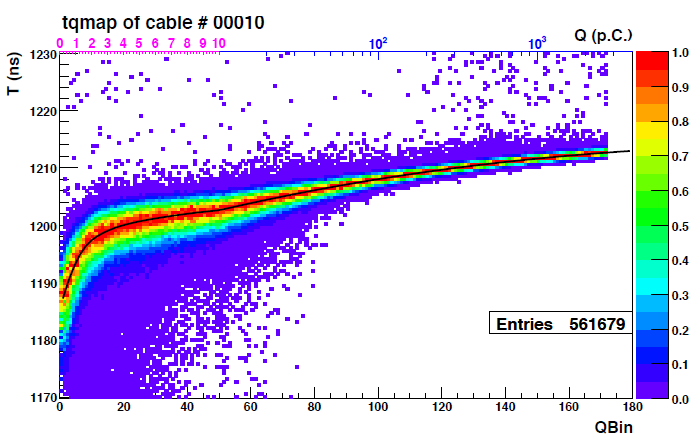
\includegraphics[width=\textwidth]{Figures/TQdist.png}
\caption{Example TQ distribution for an inner detetector PMT}
    \label{fig:TQdist}
\end{figure}


The timing resolution of the PMTs (also known as the transit time spread) is also something that must be calibrated. This is calculated by using the same timing and charge data used to produce the TQ distributions. By correcting all the ID PMT hits by their TQ distributions, these residual timing distributions have an asymmetric Gaussian function fitted to them, from which two values of sigma are extracted: $\sigma_{t}$ and $\sigma_{t'}$. These are the values for the timing resolution for before and after the peak time of this distribution. Equation \ref{eq:sigmat} shows how the asymmetric Gaussian is defined. 

\begin{align}
    f\left(t ; t>T_{\text {peak }}\right) \equiv A_{1} \cdot \exp \left(-\left(t-T_{\text {peak }}\right)^{2} / \sigma_{t}^{2}\right)+B_{1}\\
    f\left(t ; t \leq T_{\text {peak }}\right) \equiv A_{2} \cdot \exp \left(-\left(t-T_{\text {peak }}\right)^{2} / \sigma_{t}^{\prime 2}\right)+B_{2}
\label{eq:sigmat}
\end{align}

Figure \ref{fig:asygausst} shows an example of the residual timing distribution fitted with an asymmetric gaussian for a certain value of binned charge.

\begin{figure}
    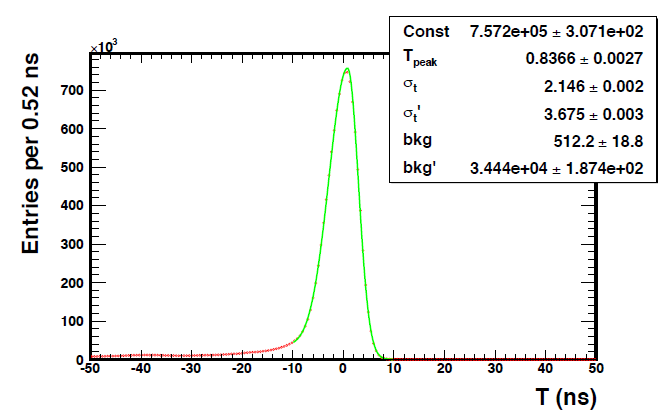
\includegraphics[width=\textwidth]{Figures/asygausst.png}
\caption{Residual timing distribution summed over all the readout channels in charge bin 14 (QBin in \ref{fig:TQdist}.)}
    \label{fig:asygausst}
\end{figure}



Figure \ref{fig:resolutiont} shows timing resolution  plotted as a function of charge for both before and after the peak time of the residual time distribution (red and blue points respectively) for SK-IV TQ calibration data. 

\begin{figure}
    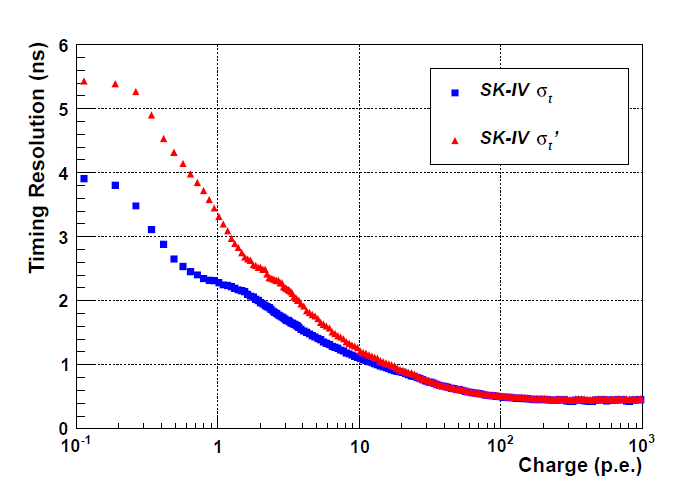
\includegraphics[width=\textwidth]{Figures/resolutiont.png}
\caption{Timing resolution as a function of charge for SK-IV}
    \label{fig:resolutiont}
\end{figure}

\subsection{Measurement of the properties of the water in Super-Kamiokande}
*to write*

\subsection{Measurement of light reflection on the black sheet and the PMTs} 

Using the same method as described in \section{Measurement of the properties of the water in Super-Kamiokande} the amount of light reflected at the PMT surface is determined. For SK-IV, four types of material, corresponding to four different refractive indices are taken into account: water, glass, bialkali, and vacuum. Table \ref{table:refractiveindex} shows the values for each of these materials, $\lambda$ is the wavelength of the light in nm and $n_{real}$ and $n_{img}$ are the real and imaginary parts of the complex refractive index.

Regarding the black sheet used to line the inside of Super-Kamiokande, it can either reflect or absorb Cherenkov photons. The amount of Cherenkov photons measured is measured by a light injector setup, shown in Figure \ref{fig:blacksheetrefsetup}. For three different incident angles of laser light ($30 \degree$, $45 \degree$ and $60 \degree$) and three different laser light wavelengths (337 nm, 400 nm and 420 nm) the charge from the light scattered off the black sheet was measured. The direct charge (i.e. the same setup without the black sheet present) was also measured, with the total black sheet reflectivity being the ratio between the scattered charge and the direct charge.

\begin{table}[H]
    $$
    \begin{array}{|cc|}
    \hline \text{Material} & \text{Refractive index} \\
    \hline Water & 1.33 \\
    \hline Glass & 1.472+3670/\lambda^{2} \\
    \hline Bi-alkali & n_{real} + i \dot n_{img} \\
    \hline Vacuum & 1.00 \\
    \hline x_{a b s}^{N} & \text { Nucleon absorption probability }  \\
    \hline x_{\pi}^{N} & \text { Nucleon } \pi \text {-production probability }\\
    \hline

    
    \end{array}
    $$
    \caption{Refractive indices of materials inside the Super-K detector.} 
    \label{table:refractiveindex}
    \end{table}
    

\begin{figure}
    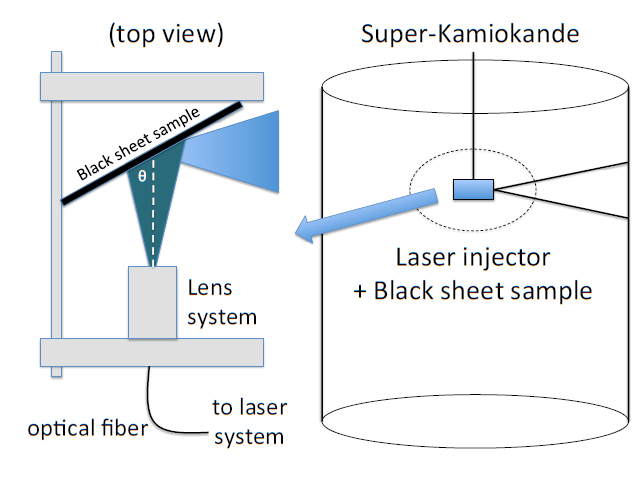
\includegraphics[width=\textwidth]{Figures/blacksheetrefsetup.png}
\caption{Schematic of the laser light reflectivity. Bird's-eye view (left) and setup inside of Super-Kamiokande (right).}
    \label{fig:blacksheetrefsetup}
\end{figure}

\subsubsection{Temperature gradient and water transparency measurements}
There is a vertical temperature gradient in the Super-Kamiokande tank due to the fact that ultrapure water is supplied upwards from the bottom of the detector shown in Figure \ref{fig:watergrad}. Below $z$ = 11m, there is no variation in temperature, whereas above this value there is an increase of temperture as height in the detector increases. This variation in temperature causes a variation in the attenuation length of light in the detector, which means that the probability of PMTs being hit changes depending on the depth in the detector. 

\begin{figure}
    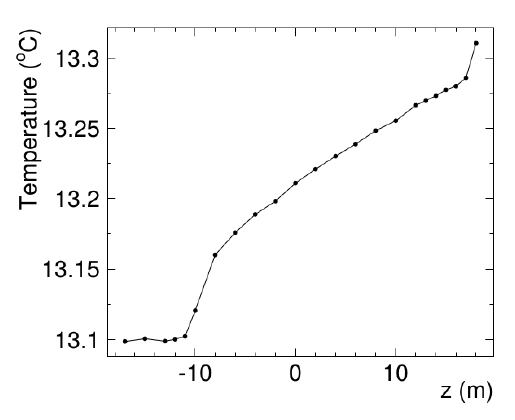
\includegraphics[width=\textwidth]{Figures/watergrad.png}
\caption{Vertical position in the detetector (z), plotted against the temperature of the water.}
    \label{fig:watergrad}
\end{figure}

Using the nickel source mentioned in the section in absolute gain calibration, the dependence between the amount of light attenuation and vertical position in the tank is calculated, with the equation for this model shown in \ref{eq:TBAeq}, where $<N_{top}>$, $<N_{bottom}>$ and $<N_{barrel}>$ are the mean rate at which the PMTs at the top, bottom and barrel regions are hit.  

\begin{equation}
    E_{\nu}=\frac{m_{\pi}^{2}-m_{\mu}^{2}}{2\left(E_{\pi}-\sqrt{E_{\pi}^{2}-m_{\pi}^{2}} \cos \theta\right)}
\label{eq:TBAeq}
\end{equation}

\subsubsection{Variation of water transparency over time}

In Super-Kamiokande, the detector medium scatters and absorbs the Cherenkov light, attenuating its wavelength. The amount of light attenuation after the light has travelled distance $l$ is given by $exp(-l/L(\lambda))$.

*to write*